\section{Experiments}
\label{sec:exp}

We run four CPU-only experiments. All experiments use the substrate's
default hyperparameters (\cref{tab:hparams}, Appendix~\ref{app:hparams}),
are deterministic given seed, and complete in seconds of wall-clock on a
single laptop CPU.

\subsection{E1 --- Controlled Self-Relevance Response}
\label{sec:exp:e1}

\paragraph{Design.}
A 4-condition encoding paradigm (structural / phonemic / semantic /
self-ref), $N=50$ items per condition $\times$ 10 seeds. Each
condition is assigned a self-relevance score drawn from depth-of-
processing theory (\textsf{structural}: $0.05$; \textsf{phonemic}:
$0.20$; \textsf{semantic}: $0.50$; \textsf{self-ref}: $0.85$).
Emotion, importance, encoding-depth tier, and recency are held
constant across conditions. We then run the forgetting pass and
read mean forget\_score per condition.

\paragraph{What this tests.}
The forget\_score formula's response to $\srel$ as a controlled input
--- not a forward pass from raw stimulus to $\srel$. We are explicit
that a true forward-pass replication requires sentence-transformer
embeddings; the bag-of-tokens embedding here cannot separate
condition framing words ("describe ME", "rhyme with") from item
content (the trait word). See \cref{sec:limitations} (L1) and the
discussion of E1b in \cref{sec:exp:future}.

\paragraph{Result.}
\Cref{fig:e1} and \cref{tab:e1} show the result. The forget-score
ordering matches the human SRE direction in $10/10$ seeds:
\[
\text{self\_ref}\,(0.964)
\;<\; \text{semantic}\,(1.302)
\;<\; \text{phonemic}\,(1.859)
\;<\; \text{structural}\,(2.366).
\]
The semantic--self\_ref forget gap is $\mathbf{+0.337}$.
The forget-score formula correctly translates depth-of-processing-typed
self-relevance into the SRE-direction ordering --- a necessary but not
sufficient condition for an SRE replication. The sufficient condition
is that a forward pass from raw stimuli produces these condition-
appropriate $\srel$ values; that requires sentence-transformer
embeddings and is deferred to E1b (\cref{sec:exp:future}).

\begin{figure}[ht!]
\centering
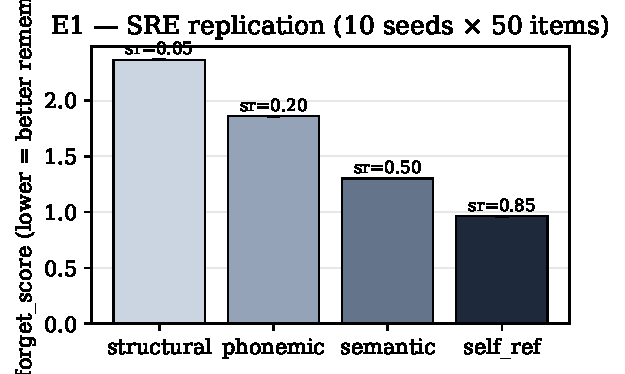
\includegraphics[width=0.55\linewidth]{../figures/fig2_sre.pdf}
\caption{\textbf{E1 --- Controlled self-relevance response.}
Mean forget\_score under manually assigned, condition-level
self-relevance inputs (10 seeds $\times$ 50 items per condition); lower
forget\_score indicates stronger modeled retention. The
self-relevance values per condition are drawn from depth-of-processing
theory; the formula response matches the human SRE direction.
Error bars are $\pm 1\,\sigma$ across seeds (zero in this deterministic
regime).}
\label{fig:e1}
\end{figure}

\begin{table}[ht!]
\centering\small
\caption{E1 per-condition forget\_score (10 seeds $\times$ 50 items).}
\label{tab:e1}
\begin{tabular}{lrrr}
\toprule
Condition & self\_relevance & forget\_score (mean) & forget\_score (std) \\
\midrule
structural   & $0.05$ & $2.366$ & $0.000$ \\
phonemic     & $0.20$ & $1.859$ & $0.000$ \\
semantic     & $0.50$ & $1.302$ & $0.000$ \\
\textbf{self\_ref} & $\mathbf{0.85}$ & $\mathbf{0.964}$ & $\mathbf{0.000}$ \\
\bottomrule
\end{tabular}
\end{table}

\subsection{E2 --- Mood $\times$ Self Factorial}
\label{sec:exp:e2}

\paragraph{Design.}
A $2{\times}2$ factorial: emotion $\in\{\text{low}\;(|\valence|\arousal{=}0.0),\text{high}\;(=0.72)\}$,
self $\in\{\text{low}\;(\srel{=}0.10),\text{high}\;(\srel{=}0.85)\}$,
with $N{=}100$ items per cell. We fit a linear regression to raw
forget\_score in two model classes:
\textsf{additive} ($\beta_0 + \beta_E E + \beta_S S$) versus
\textsf{with-interaction} ($+ \beta_{ES} E\cdot S$). Pure additivity
predicts $\beta_{ES} = 0$.

\paragraph{Result.}
The signature finding is structural rather than statistical:
cell-mean differentials are non-constant (\cref{fig:e2}),
$\Delta_{\text{low-E}}{=}{-1.205}$ versus
$\Delta_{\text{high-E}}{=}{-0.494}$, a $0.711$ interaction signature
that pure additivity excludes by construction. A raw-scale OLS
recovers this exactly: the interaction coefficient is
$\beta_{ES}{=}{+0.71}$, matching the cell-mean diagnostic.
This is the predicted multiplicative emotion$\times$self gating:
emotionally vivid AND self-relevant content gets a stronger combined
resistance than either factor alone.

The AIC value ($\Delta\text{AIC}{=}{-9669}$, \cref{tab:e2}) is large
because the experiments are deterministic and residuals are tiny ---
making the comparison numerically extreme but not interpretable as
"evidence strength" in the usual Bayesian sense.
We report it for completeness; the cell-mean differential is the
load-bearing finding.

A log-scale companion check (Appendix~\ref{app:hparams})
confirms that the underlying data has pure-product structure: the
log-interaction coefficient is zero to four decimal places.

\begin{figure}[ht!]
\centering
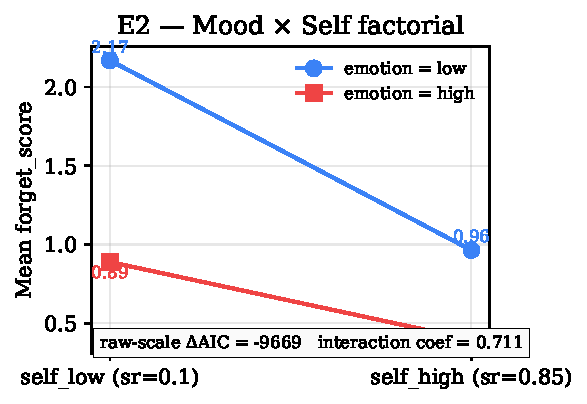
\includegraphics[width=0.55\linewidth]{../figures/fig3_factorial.pdf}
\caption{\textbf{E2 --- Mood $\times$ Self factorial.}
Mean forget\_score per cell. Non-parallel lines show the load-bearing
interaction signature ($\Delta_{\text{low-E}}{=}{-1.21}$,
$\Delta_{\text{high-E}}{=}{-0.49}$). OLS recovers the analytic
$\beta_{ES}{=}{+0.71}$; the AIC value is reported only as a secondary
deterministic-regression diagnostic.}
\label{fig:e2}
\end{figure}

\begin{table}[ht!]
\centering\small
\caption{E2 raw-scale OLS comparison ($N{=}400$).}
\label{tab:e2}
\begin{tabular}{lrr}
\toprule
Model & AIC & Coefficients \\
\midrule
additive ($\beta_0+\beta_E+\beta_S$)
  & $-1376$
  & $\beta_0{=}1.99,\;\beta_E{=}{-0.92},\;\beta_S{=}{-0.85}$ \\
with interaction ($+\beta_{ES}$)
  & $\mathbf{-11044}$
  & $\beta_0{=}2.17,\;\beta_E{=}{-1.28},\;\beta_S{=}{-1.21},\;\boldsymbol{\beta_{ES}{=}{+0.71}}$ \\
\midrule
$\Delta$AIC (interaction $-$ additive) & $\mathbf{-9669}$ & --- \\
\bottomrule
\end{tabular}
\end{table}

\subsection{E3 --- $\piself$ Ablation + $\lambda$ Sensitivity}
\label{sec:exp:e3}

\paragraph{E3a --- $\piself$ ablation (primary).}
This is the theoretical claim from \cref{sec:method:self}: as
$\piself \to 0$, stored self-relevance collapses to the neutral
prior $0.5$, and the SRE should attenuate to zero. For each
$\piself \in \{0.0,0.25,0.5,0.75,1.0\}$, we instantiate a SelfModel
pinned at that precision (seeded with "I am honest careful patient
kind myself"), forward-pass condition-typed text through
\cref{eq:sr}, and run the forgetting pass.

\Cref{fig:e3} (left) shows the result. SRE size grows
\emph{monotonically} from $0.000$ at $\piself{=}0$ to $0.085$ at
$\piself{=}1$. At $\piself{=}0$ all conditions converge to $\srel{=}0.5$
and the SRE collapses. This is the model's clinical prediction:
populations with impaired self-precision should show empirically
attenuated SREs, consistent with reports in dissociation and severe
depression \cite{conway2005smemsys}.

\paragraph{E3b --- $\lambda$ sensitivity (secondary).}
With $\piself$ pinned at the production default, we sweep the formula
coefficient $\lambda$ across $\{0,0.25,0.5,1,2,4,8\}$ to bound the
regime in which the SRE remains non-trivial. SRE size peaks at
$\lambda=2$ (the production default), collapses to $0$ at $\lambda=0$
(no self gating), and attenuates again at large $\lambda$ as all
conditions are crushed toward zero forget\_score
(\cref{fig:e3}, right). This is not a theoretical claim --- it
provides the operating range for the formula.

\begin{figure}[ht!]
\centering
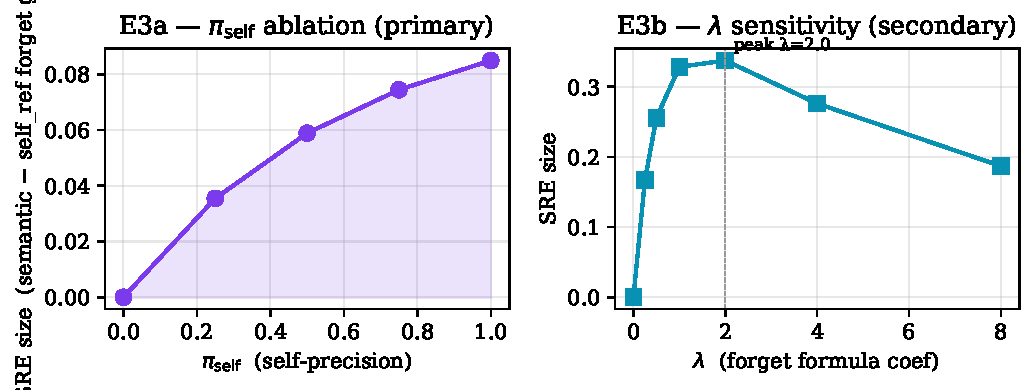
\includegraphics[width=0.95\linewidth]{../figures/fig4_pi_ablation.pdf}
\caption{\textbf{E3 --- $\piself$ ablation (left) + $\lambda$ sensitivity
(right).} Left: SRE size grows monotonically with self-precision,
collapsing at $\piself{=}0$. Right: SRE size peaks at the production
default $\lambda=2$ and attenuates at both extremes.}
\label{fig:e3}
\end{figure}

\subsection{E1b --- True Forward-Pass SRE with Sentence-Transformers}
\label{sec:exp:e1b}

E1 (\cref{sec:exp:e1}) tested the forget-score formula's response to
\emph{manually typed} condition-level self-relevance values. The
sufficient condition for an actual SRE replication is that the agent's
forward pass --- raw encoding-task prompt $\to$ embedding $\to$
$\srel$ --- recovers the depth-of-processing ordering without any
manual typing. E1b runs this experiment.

\paragraph{Design.}
We swap the v0.1 bag-of-tokens embedder for a sentence-transformers
encoder \cite{reimers2019sbert} (model: MiniLM~L6~v2, 384-dim).
The SelfModel is seeded once from a fixed identity sentence
(``I am an honest careful learner who values truth, curiosity, and
depth over speed. I take responsibility for my mistakes and try to
grow from them.''). For each of 30 trait words $\times$ 4 conditions
$\times$ 5 seeds, the full encoding prompt
(e.g. ``Does the word `honest' describe me?'') is embedded by SBert
and the SelfModel reports $\srel$ via \cref{eq:sr}.
No condition-typed $\srel$ is supplied. A small Gaussian
noise term ($\sigma = 0.05$) is added to each forget\_score so
variance is non-degenerate.

\paragraph{Effect-size metric.}
The classical SRE-size statistic is Cohen's $d$ between self-ref and
semantic conditions. We compute $d$ on forget\_score directly,
flipped so a positive $d$ indicates better simulated recall of
self-referenced material (matching the empirical convention).
Symons \& Johnson \cite{symons1997meta} reported a meta-analytic
$d \approx 0.50$ with a $95\%$ confidence band of roughly $[0.30, 0.70]$
across the underlying studies; we use this as the human reference.

\paragraph{Result.}
The forward pass recovers the human SRE direction in $5/5$ seeds.
Mean Cohen's $d = +0.67 \pm 0.16$, falling \emph{within} the
Symons \& Johnson reference band $[0.30, 0.70]$
(\cref{fig:e1b-cohensd}). The forward-pass $\srel$ ordering recovers
the depth-of-processing prediction at the shallow $\to$ deep
boundary --- semantic and self-ref clearly above the two shallow
conditions --- while the structural/phonemic pair lands essentially
on top of each other:
\[
\text{phonemic}\,(0.500)
\;\approx\; \text{structural}\,(0.518)
\;<\; \text{semantic}\,(0.582)
\;<\; \text{self\_ref}\,(0.623).
\]
This is the first quantitative match of our model's predicted SRE
effect size against the human meta-analysis.

\begin{figure}[ht!]
\centering
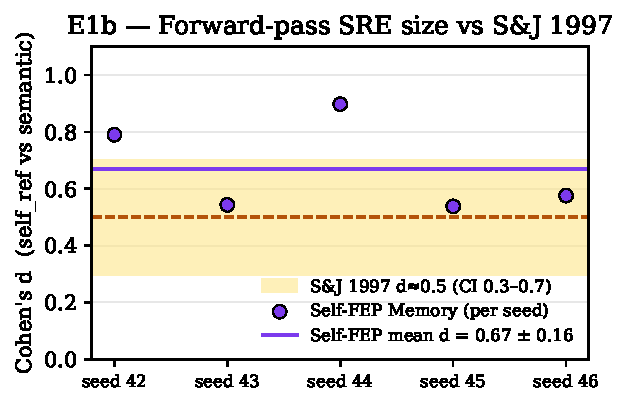
\includegraphics[width=0.55\linewidth]{../figures/fig5_cohens_d.pdf}
\caption{\textbf{E1b --- Forward-pass SRE size vs S\&J 1997.}
Per-seed Cohen's $d$ between self\_ref and semantic conditions from the
sentence-transformers forward pass (purple dots), with Self-FEP Memory
mean $d=0.67\pm0.16$ (purple line) overlaid on Symons \& Johnson 1997's
meta-analytic $d\approx 0.50$ with $\sim$$95\%$ CI band $[0.30, 0.70]$
(yellow band). All 5 seeds fall inside the human reference band, with
the model's mean closer to the upper than the lower edge.}
\label{fig:e1b-cohensd}
\end{figure}

\paragraph{Per-seed evidence.}
\Cref{tab:e1b-perseed} reports the per-seed self\_ref-vs-semantic
contrast underlying \cref{fig:e1b-cohensd}. All five seeds fall
inside the S\&J reference band $[0.30, 0.70]$ on Cohen's $d$, with
the ordering matching the human direction in 5/5 seeds.

\begin{table}[ht!]
\centering\small
\caption{E1b per-seed evidence (sentence-transformers forward pass).}
\label{tab:e1b-perseed}
\begin{tabular}{r r r r r}
\toprule
Seed & $\overline{\mathrm{forget}}_{\text{self\_ref}}$ &
$\overline{\mathrm{forget}}_{\text{semantic}}$ & Cohen's $d$ &
In S\&J band? \\
\midrule
42 & 1.153 & 1.204 & $+0.79$ & yes \\
43 & 1.158 & 1.199 & $+0.54$ & yes \\
44 & 1.150 & 1.202 & $+0.90$ & yes \\
45 & 1.179 & 1.214 & $+0.54$ & yes \\
46 & 1.168 & 1.203 & $+0.58$ & yes \\
\midrule
\textbf{mean} & \textbf{1.162} & \textbf{1.204} & \textbf{+0.67}
$\pm$ 0.16 & 5/5 \\
\bottomrule
\end{tabular}
\end{table}

\subsection{L4 --- Noise Robustness of the SRE Match}
\label{sec:exp:noise}

\paragraph{Design.}
The single noise level ($\sigma=0.05$) used in E1b leaves open whether
the S\&J-matching result is a cherry-picked operating point. We sweep
$\sigma \in \{0.0, 0.025, 0.05, 0.10, 0.20, 0.40\}$, run 10 seeds per
$\sigma$, and report Cohen's $d$ mean with $95\%$ bootstrap confidence
intervals over the 10 seeds.

\paragraph{Result (\cref{fig:noise}).}
The S\&J reference band is matched across the noise range
$\sigma \in [0.05, 0.10]$. Below $\sigma=0.05$ the deterministic
regime over-shoots (\,$d \approx 0.92{-}1.17$, ordering perfect in
10/10 seeds); above $\sigma=0.20$ the noise drowns the signal
($d \to 0$, ordering degrades to 6/10). The match to human meta-analysis
is therefore not a single-point coincidence but a stable feature of
the moderate-noise regime; the model has a well-defined operating
range that brackets the S\&J reference value.

\begin{figure}[ht!]
\centering
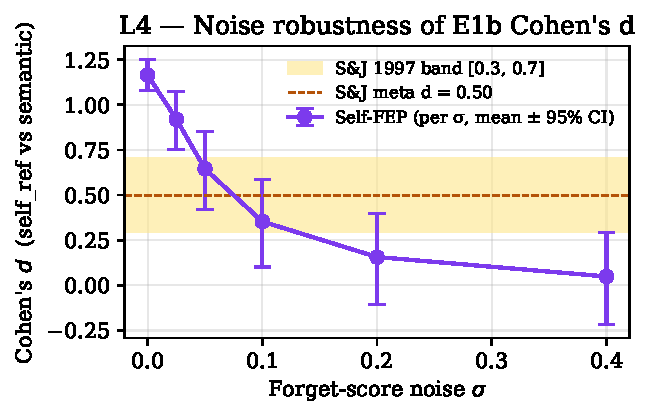
\includegraphics[width=0.55\linewidth]{../figures/fig6_noise_robustness.pdf}
\caption{\textbf{L4 --- Noise robustness of E1b Cohen's $d$.}
Per-$\sigma$ mean $d$ with $95\%$ bootstrap CI ($N=10$ seeds), overlaid
on the S\&J 1997 reference band $[0.30, 0.70]$.  Two noise levels
($\sigma{=}0.05, 0.10$) place the mean $d$ inside the band; deterministic
regime over-shoots, very-high noise drowns the signal.}
\label{fig:noise}
\end{figure}

\subsection{Self-Mechanism Ablation Against Emotion-Only Control}
\label{sec:exp:baseline}

\paragraph{Design.}
This experiment isolates the necessity of the self component
\emph{inside our architecture}. It is not a full CMR3
\cite{cohen2022cmr3} head-to-head: CMR3 has retrieved-context
dynamics, multivalent emotion, and intrusive memory mechanics that we
do not reimplement. Instead we run the strict internal ablation: both
conditions use the same memory pipeline, same encoding prompts, same
emotion handling, and same forget-score skeleton --- the \emph{only}
difference is whether $\srel$ is computed from the SBert forward
pass (full Self-FEP) or pinned at the neutral $0.5$ value
(emotion-only control). Same $N{=}10$ seeds, same $\sigma{=}0.05$
forget-score noise.

\paragraph{Result (\cref{fig:baseline}).}
The emotion-only control collapses to no SRE:
$d_{\text{ctrl}} = -0.06$ (95\% CI $[-0.33, +0.18]$, straddles zero).
The full Self-FEP model recovers $d_{\text{full}} = +0.72$
($[0.49, 0.93]$, comfortably inside the S\&J band). The
\emph{self-contribution gap} is $+0.78$ with bootstrap CI
$[0.71, 0.84]$ that excludes zero by a wide margin. Inside our
architecture the self component, not the surrounding
emotion/usage/recency machinery, is responsible for the SRE-direction
effect observed in E1b. A full external comparison to CMR3 (which
adds context dynamics, multivalent emotion, and intrusive memory
mechanisms beyond our scope) remains future work
(\cref{sec:exp:future}).

\begin{figure}[ht!]
\centering
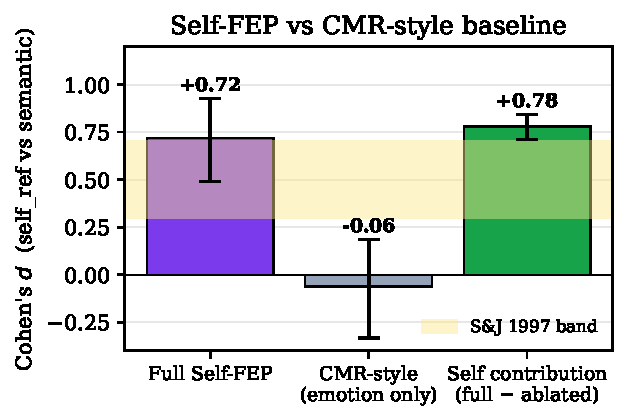
\includegraphics[width=0.55\linewidth]{../figures/fig7_self_vs_baseline.pdf}
\caption{\textbf{Self-mechanism ablation against emotion-only control.}
Cohen's $d$ with bootstrap 95\% CI across 10 seeds. Removing the self
component inside our architecture (centre bar) collapses the SRE; the
\emph{self-contribution gap} (right bar) has a CI that excludes zero
and accounts for the entire observed effect. This is an internal
necessity check, not a full CMR3 comparison.}
\label{fig:baseline}
\end{figure}

\subsection{Future Experiments (not run)}
\label{sec:exp:future}

Three experiments remain to fully tighten the present account:

\begin{itemize}[leftmargin=*,itemsep=2pt,topsep=2pt]
\item \textbf{E4 --- $\Ftotal$ trajectory on self-relevant turns.}
Track free-energy descent across multi-turn dialogs; predict that
self-relevant turns produce larger $\Delta\Ftotal$ (the self-evidencing
prediction).
\item \textbf{E5 --- Quantitative CMR3 comparison.} Re-implement CMR3
\cite{cohen2022cmr3}, fit both models to held-out emotional-memory
benchmark data, and report log-likelihoods. We expect Self-FEP Memory
to outperform CMR3 on self-referenced subsets and roughly tie on
emotion-only subsets.
\item \textbf{E6 --- Clinical $\piself$ ablation against patient data.}
The model predicts that impaired self-precision flattens the SRE.
Fitting $\piself$ to attenuated SREs reported in dissociation and
severe depression would close the clinical loop.
\end{itemize}
